%This is my super simple Real Analysis Homework template

\documentclass{article}
\usepackage[utf8]{inputenc}
\usepackage[english]{babel}
\usepackage[]{amsthm} %lets us use \begin{proof}
\usepackage[]{amssymb} %gives us the character \varnothing
\usepackage{graphicx}
\usepackage{hyperref}


\title{Homework 1}
\author{Aasim Zahoor}
\date\today
%This information doesn't actually show up on your document unless you use the maketitle command below

\begin{document}
\maketitle %This command prints the title based on information entered above

%Section and subsection automatically number unless you put the asterisk next to them.
\begin{center}
\section{Problems}
\end{center}
\textbf{Link}\vspace{1.5em}
\url{https://github.com/AasimZahoor/Comp_methods.git}
\vspace{1.5em}

\textbf{Problem 1}\vspace{1.5em}

In my code, I have defined three functions, one for bisection, one for secant and one for Newton's. Arguments for the bisection and the secant method are the range, the function and threshold. Arguments for the  Newton's method is the initial guess, the function, derivative of the function and the threshold.  All of them have a default threshold value of $10^{-6}$. All three of them return the final value and the number of iterations it took to reach that value(in a tuple).

\vspace{1.5em}
\textbf{Problem 2}\vspace{1.5em}

For this problem I wrote a code where I defined two functions, one gives the column density for pseudo-isothermal sphere as output and one gives the derivative of the column density as the output. I also hardcoded a set of threshold values and then made the code calculate width at half maximum for each method and each threshold value and plotted it.
\vspace{1.5em}
\begin{center}
 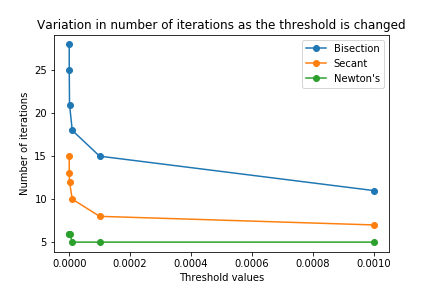
\includegraphics[scale=0.3]{Images/HW1_pb2}
 \end{center}
 
\vspace{5em}
\textbf{Problem 3}
\vspace{1.5em}

For this problem I divided time of one year into 12 months and used a for loop to find the location of the observer at each month. I called the bisection method for each observer position which gave me the lens plane x value. The gaussian lens equation is obtained by calling the f function.
\vspace{1.5em}
\begin{center}
 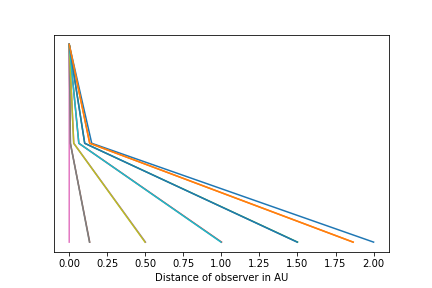
\includegraphics[scale=0.3]{Images/HW_1_pb3}
 \end{center}
 
\vspace{1.5em}
 
\textbf{Problem 4}\vspace{1.5em}

Same as problem 3 but now the f function gives out the pseudo isothermal equation.
\vspace{1.5em}
\begin{center}
 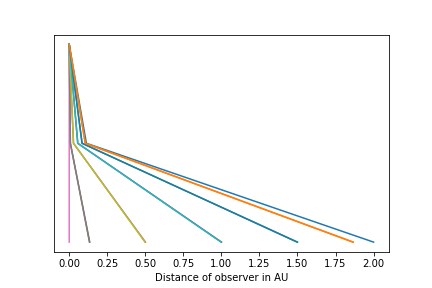
\includegraphics[scale=0.3]{Images/HW_1_pb4}
 \end{center}
 
\vspace{1.5em}

\textbf{Problem 5}\vspace{1.5em}

I made a function which takes in the x and y points and the x points we are interested in and gives the y values as output.
\vspace{1.5em}

\textbf{Problem 6}\vspace{1.5em}

I used the interpolator I defined in problem $5$ and gave it the x and y values taken from lensdensity.txt and the x values we are interested in and got the corresponding y values as output. I used the x and y values to draw a plot.  
\vspace{1.5em}
\begin{center}
 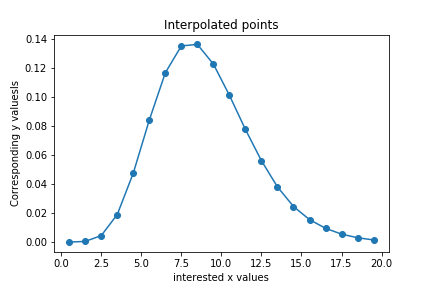
\includegraphics[scale=0.3]{Images/HW_1_pb6}
 \end{center}
 
\vspace{1.5em}

\end{document}